\chapter{Simpleks -- Perhitungan Matriks}
\label{ch:simplex-matrix}

Pada bab sebelumnya, kita menjalankan metode simpleks melalui kamus: tulis ulang, lakukan pivot, ulangi.  Sudut pandang tersebut baik untuk membangun intuisi.  Dalam bab ini, kita menguraikan \emph{aljabar linear} yang mendasarinya.  Setiap kamus yang Anda tulis merupakan pernyataan tentang matriks: memilih basis berarti memilih submatriks $A_B$ yang dapat diinvers, melakukan pivot berarti mengganti submatriks tersebut, dan baris objektif suatu kamus merupakan vektor \emph{biaya tereduksi} yang dihitung dari $A_B^{-1}$.  Perumusan yang presisi ini menjelaskan \emph{mengapa} metode tersebut bekerja, sekaligus menunjukkan bagaimana simpleks diimplementasikan dalam perangkat lunak, tempat solver memanipulasi matriks basis alih-alih menulis ulang persamaan.

Kita melanjutkan dalam dua tahap.  Bagian~\ref{sec:solutions-axb} menunjukkan bagaimana pemartisian variabel ke dalam himpunan basis dan nonbasis mengubah $A\x = \b$ menjadi rumus untuk solusi basis.  Bagian~\ref{sec:optimality-conditions} kemudian menuliskan ulang objektif dari sudut pandang suatu basis sehingga diperoleh sertifikat optimalitas secara aljabar.

\section{Solusi untuk $A\x = \b$}
\label{sec:solutions-axb}
\begin{outcome}
\begin{itemize}
\item Menyelidiki cara menuliskan ulang suatu sistem persamaan melalui pemartisian variabel
\item Melihat cara memartisi matriks dan menuliskan ulang persamaan dalam bentuk baru yang menyelesaikan variabel basis
\item Membiasakan diri dengan notasi matriks
\item Mendefinisikan istilah solusi basis dan solusi basis layak
\end{itemize}
\end{outcome}
Sekarang kita akan menyelidiki berbagai cara untuk merepresentasikan solusi sistem persamaan linear ini.  Pembahasan ini memberikan landasan teoretis bagi algoritma simpleks.  

Kita tinjau suatu sistem linear

$$
A \mathbf{x} = \mathbf{b},
$$

dengan $A \in \mathbb{R}^{m \times n}$, $\mathbf{x} \in \mathbb{R}^n$, dan $\mathbf{b} \in \mathbb{R}^m$. Secara eksplisit,

$$
A =
\begin{bmatrix}
    a_{11} & \cdots & a_{1n} \\
    \vdots & \ddots & \vdots \\
    a_{m1} & \cdots & a_{mn}
\end{bmatrix}, \quad
\mathbf{x} =
\begin{bmatrix}
    x_1 \\
    \vdots \\
    x_n
\end{bmatrix}, \quad
\mathbf{b} =
\begin{bmatrix}
    b_1 \\
    \vdots \\
    b_m
\end{bmatrix}.
$$

\subsection*{Asumsi tentang $A$}

Kita mengasumsikan:
\begin{itemize}
\item $\text{rank}(A) = m$, yaitu baris-baris $A$ saling bebas linear (berperingkat baris penuh);
\item $m \leq n$, sehingga sistem tidak memiliki terlalu banyak persamaan.
\end{itemize}

Jika $A$ tidak berperingkat baris penuh, sebagian persamaan akan redundan dan dapat dihilangkan tanpa mengubah himpunan solusi. Ketika $m > n$, sistem biasanya memiliki terlalu banyak persamaan dan tidak konsisten; jika konsisten, sistem tersebut dapat direduksi menjadi $m \leq n$ melalui operasi baris.

Di bawah asumsi ini, $A\mathbf{x} = \mathbf{b}$ merepresentasikan sistem yang terdiri atas $m$ persamaan bebas dalam $n$ variabel tak diketahui, dengan ruang solusi yang layak (dan mungkin tak hingga).

\subsubsection{Contoh Masalah -- Toko Roti Kecil}
\label{sec:bakery-problem}

Sebuah toko roti kecil menghasilkan dua produk: \emph{roti tawar} (dinyatakan dengan \(x\)) dan \emph{kue} (dinyatakan dengan \(y\)). Setiap roti tawar memberikan laba \$2, sedangkan setiap kue memberikan laba \$3. Toko roti tersebut harus beroperasi dengan kendala harian berikut:

\begin{itemize}
    \item \textbf{Waktu Oven:} Karena waktu oven terbatas, jumlah keseluruhan roti tawar dan kue yang dipanggang setiap hari tidak boleh melebihi 9. Hal ini memberikan kendala:
    \[
    x + y \leq 9.
    \]
    
    \item \textbf{Persediaan Tepung:} Roti tawar menggunakan lebih banyak tepung daripada kue. Setiap roti tawar menggunakan 2 satuan tepung dan setiap kue menggunakan 1 satuan. Toko roti memiliki paling banyak 16 satuan tepung setiap hari, sehingga diperoleh:
    \[
    2x + y \leq 16.
    \]
    
    \item \textbf{Persediaan Gula:} Kue menggunakan lebih banyak gula daripada roti tawar. Setiap roti tawar menggunakan 1 satuan gula dan setiap kue menggunakan 2 satuan. Persediaan gula harian terbatas pada 14 satuan, sehingga:
    \[
    x + 2y \leq 14.
    \]

    \item \textbf{Nonnegativitas:} Toko roti tidak dapat memproduksi barang dalam jumlah negatif, sehingga:
    \[
    x \geq 0, \quad y \geq 0.
    \]
\end{itemize}

\modelhead{Model}

Toko roti ingin menentukan jumlah roti tawar (\(x\)) dan kue (\(y\)) yang harus diproduksi setiap hari untuk memaksimumkan laba total. Program linear yang dihasilkan adalah:

\begin{tcolorbox}[colback=orange!5!white, colframe=orange!75!black,    
    width=0.6\textwidth, % adjust width as desired
    box align=center, 
    title=\textbf{Program Linear Awal}]
\[
\begin{aligned}
\max \quad & 2x + 3y \\
\st \quad 
& x + y \leq 9  & \text{(jam)}\\
& 2x + y \leq 16  & \text{(tepung)}\\
& x + 2y \leq 14 & \text{(gula)}\\
& x \geq 0,\; y \geq 0.
\end{aligned}
\]
\end{tcolorbox}

Kita mulai dengan menambahkan \emph{variabel slack} \( s_1, s_2, s_3 \) untuk mengubah pertidaksamaan menjadi persamaan:

\begin{tcolorbox}[colback=gray!5!white, colframe=gray!75!black,    
    width=0.6\textwidth, % adjust width as desired
    box align=center, 
    title=\textbf{Bentuk Standar}]
\[
\begin{aligned}
\max \quad & 2x + 3y \\
\st \quad 
&x + y + s_1 = 9 \quad &\text{(jam)} \\
&2x + y + s_2 = 16 \quad &\text{(tepung)} \\
&x + 2y + s_3 = 14 \quad &\text{(gula)} \\
&x, y, s_1, s_2, s_3 \geq 0
\end{aligned}
\]
\end{tcolorbox}

Kita juga perlu memahami bentuk standar dari sudut pandang matriks.

\begin{tcolorbox}[colback=gray!5!white, colframe=gray!75!black,    
    width=0.8\textwidth, % adjust width as desired
    box align=center, 
    title=\textbf{Bentuk Standar Matriks--Vektor}]
\noindent Dalam notasi matriks--vektor, definisikan:
\[
\mathbf{x} = 
\begin{bmatrix}
x \\
y \\
s_1 \\
s_2 \\
s_3
\end{bmatrix},
\quad
\mathbf{c} =
\begin{bmatrix}
2 \\
3 \\
0 \\
0 \\
0
\end{bmatrix},
\quad
A =
\begin{bmatrix}
1 & 1 & 1 & 0 & 0 \\
2 & 1 & 0 & 1 & 0 \\
1 & 2 & 0 & 0 & 1
\end{bmatrix},
\quad
\mathbf{b} =
\begin{bmatrix}
9 \\
16 \\
14
\end{bmatrix}
\]

\bigskip

\noindent Dengan demikian, program linear bentuk standarnya adalah:
\[
\begin{aligned}
\max \quad & \mathbf{c}^\top \mathbf{x} \\
\st \quad & A\mathbf{x} = \mathbf{b}, \\
& \mathbf{x} \geq \mathbf{0}
\end{aligned}
\]

\end{tcolorbox}

\subsection*{Notasi Submatriks}
Kita mengambil submatriks dari \( A \) dengan memilih kolom-kolom yang bersesuaian dengan himpunan variabel tertentu.  
Untuk suatu himpunan \( I \), kita menggunakan \( A_I \) untuk menyatakan submatriks dari \( A \) yang bersesuaian dengan kolom-kolom dalam \( I \).

\bigskip

\[
\begin{array}{c}
\begin{array}{ccccc}
\scriptstyle x & \scriptstyle y & \scriptstyle s_1 & \scriptstyle s_2 & \scriptstyle s_3
\end{array} \\
\left[
\begin{array}{>{\columncolor{yellow}}c c c c c}
1 & 1 & 1 & 0 & 0 \\
2 & 1 & 0 & 1 & 0 \\
1 & 2 & 0 & 0 & 1
\end{array}
\right]
\end{array}
\quad
\Rightarrow
\quad
A_{\{x\}} =
\begin{bmatrix}
1 \\
2 \\
1
\end{bmatrix}
\]

\bigskip

\[
\begin{array}{c}
\begin{array}{ccccc}
\scriptstyle x & \scriptstyle y & \scriptstyle s_1 & \scriptstyle s_2 & \scriptstyle s_3
\end{array} \\
\left[
\begin{array}{c>{\columncolor{cyan}}c c >{\columncolor{cyan}}c c}
1 & 1 & 1 & 0 & 0 \\
2 & 1 & 0 & 1 & 0 \\
1 & 2 & 0 & 0 & 1
\end{array}
\right]
\end{array}
\quad
\Rightarrow
\quad
A_{\{y, s_2\}} =
\begin{bmatrix}
1 & 0 \\
1 & 1 \\
2 & 0
\end{bmatrix}
\]
\bigskip

\[
\begin{array}{c}
\begin{array}{ccccc}
\scriptstyle x & \scriptstyle y & \scriptstyle s_1 & \scriptstyle s_2 & \scriptstyle s_3
\end{array} \\
\left[
\begin{array}{c c >{\columncolor{orange}}c >{\columncolor{orange}}c >{\columncolor{orange}}c}
1 & 1 & 1 & 0 & 0 \\
2 & 1 & 0 & 1 & 0 \\
1 & 2 & 0 & 0 & 1
\end{array}
\right]
\end{array}
\quad
\Rightarrow
\quad
A_{\{s_1, s_2, s_3\}} =
\begin{bmatrix}
1 & 0 & 0 \\
0 & 1 & 0 \\
0 & 0 & 1
\end{bmatrix}
\]

\bigskip

\begin{align*}
A\mathbf{x}
&=
\begin{bmatrix}
1 & 1 & 1 & 0 & 0 \\
2 & 1 & 0 & 1 & 0 \\
1 & 2 & 0 & 0 & 1
\end{bmatrix}
\begin{bmatrix}
x \\ y \\ s_1 \\ s_2 \\ s_3
\end{bmatrix}
=
\begin{bmatrix}
1x + 1y + 1s_1 \\
2x + 1y + 1s_2 \\
1x + 2y + 1s_3
\end{bmatrix} \\
&=
\underbrace{
\begin{bmatrix}
1 & 1 \\
2 & 1 \\
1 & 2
\end{bmatrix}
\begin{bmatrix}
x \\ y
\end{bmatrix}
}_{A_{\{x,y\}} (x, y)}
+
\underbrace{
\begin{bmatrix}
1 & 0 & 0 \\
0 & 1 & 0 \\
0 & 0 & 1
\end{bmatrix}
\begin{bmatrix}
s_1 \\ s_2 \\ s_3
\end{bmatrix}
}_{A_{\{s_1,s_2,s_3\}} (s_1, s_2, s_3)}
\end{align*}

\bigskip

\begin{align*}
A\mathbf{x}
&=
\underbrace{
\begin{bmatrix}
1 & 1 & 0 \\
2 & 1 & 1 \\
1 & 2 & 0
\end{bmatrix}
\begin{bmatrix}
x \\ y \\ s_2
\end{bmatrix}
}_{A_{\{x, y, s_2\}} (x, y, s_2)}
+
\underbrace{
\begin{bmatrix}
1 & 0 \\
0 & 0 \\
0 & 1
\end{bmatrix}
\begin{bmatrix}
s_1 \\ s_3
\end{bmatrix}
}_{A_{\{s_1, s_3\}} (s_1, s_3)}
=
\begin{bmatrix}
9 \\ 16 \\ 14
\end{bmatrix}
\end{align*}

\bigskip

Hal ini menyiratkan:

\begin{align*}
A_{\{x, y, s_2\}} 
\begin{bmatrix}
x \\ y \\ s_2
\end{bmatrix}
&=
\begin{bmatrix}
9 \\ 16 \\ 14
\end{bmatrix}
-
A_{\{s_1, s_3\}}
\begin{bmatrix}
s_1 \\ s_3
\end{bmatrix}
\end{align*}

\bigskip

Dengan demikian,

\begin{align*}
\begin{bmatrix}
x \\ y \\ s_2
\end{bmatrix}
&=
A_{\{x, y, s_2\}}^{-1}
\left(
\begin{bmatrix}
9 \\ 16 \\ 14
\end{bmatrix}
-
A_{\{s_1, s_3\}}
\begin{bmatrix}
s_1 \\ s_3
\end{bmatrix}
\right)
\end{align*}

\subsection{Mempartisi Variabel}

Dalam menyelesaikan sistem \( A\x =\b\) pada konteks pemrograman linear, kita memperkenalkan konsep \textbf{pemartisian variabel}. Pendekatan ini sangat penting dalam Metode Simpleks untuk mengidentifikasi dan menganalisis solusi basis.

\begin{definition}{Basis}{}
Diberikan matriks $A$ berperingkat baris penuh $m$, suatu \emph{basis} $B$ adalah himpunan indeks untuk $m$ dari $n$ kolom, sedemikian sehingga $m$ kolom matriks $A$ yang bersesuaian saling bebas linear.  Selanjutnya, kita membentuk submatriks $A_B$ yang hanya memuat kolom-kolom tersebut dari $A$. 

 Sisa \( n - m \) kolom disebut kolom \emph{nonbasis}, yang membentuk matriks \( A_N \). 
 \end{definition}
 
 Diberikan suatu basis $B$ dan himpunan nonbasis $N$, pemartisian ini membagi vektor variabel \( \x \) menjadi dua himpunan:
\[
\x =
\begin{bmatrix}
    \x_B \\ \x_N
\end{bmatrix},
\]
dengan:
\begin{itemize}
\item  \( \x_B \) terdiri atas \textbf{variabel basis}, yang terkait dengan matriks basis \( A_B \),
\item\( \x_N \) terdiri atas \textbf{variabel nonbasis}, yang terkait dengan matriks nonbasis \( A_N \).
\end{itemize}

Menuliskan ulang sistem \( A\x =\b\) berdasarkan partisi tersebut menghasilkan:
\begin{equation}
A_B \x_B + A_N \x_N = b.
\end{equation}

Jika matriks basis \( A_B \) dapat diinvers, kita dapat menyatakan \( \x_B \) dalam \( \x_N \):
\begin{equation}
\x_B = A_B^{-1}\b- A_B^{-1} A_N \x_N.
\end{equation}

\begin{definition}{Solusi Basis dan Solusi Basis Layak (BFS)}{}
Suatu \textbf{solusi basis} diperoleh dengan menetapkan \( \x_N = 0 \), sehingga:
\begin{equation}
\x_B = A_B^{-1} \b, \quad \x_N = 0.
\end{equation}

Suatu \textbf{solusi basis layak} (BFS) adalah solusi basis yang memenuhi kendala nonnegativitas \( \x_B \geq \0 \), sehingga semua variabel basis bernilai nonnegatif.
\end{definition}
\subsubsection*{Contoh 1: Sistem dengan 3 Variabel dan 2 Persamaan}

Tinjau sistem berikut:
\[
\begin{aligned}
    x_1 + 2x_2 + x_3 &= 4, \\
    3x_1 + x_2 + 2x_3 &= 5.
\end{aligned}
\]
Di sini, matriks \( A \) dan vektor variabel \( x \) adalah:
\[
A =
\begin{bmatrix}
    1 & 2 & 1 \\
    3 & 1 & 2
\end{bmatrix}, \quad
x =
\begin{bmatrix}
    x_1 \\ x_2 \\ x_3
\end{bmatrix}, \quad
b =
\begin{bmatrix}
    4 \\ 5
\end{bmatrix}.
\]
Dengan memilih \(B= \{1, 2\} \) sebagai basis, submatriks yang bersesuaian adalah:
\[
A_B =
\begin{bmatrix}
    1 & 2 \\
    3 & 1
\end{bmatrix}, \quad A_N =
\begin{bmatrix}
    1 \\
    2
\end{bmatrix}.
\]
Jika \( A_B \) dapat diinvers, kita hitung:
\[
A_B^{-1} =
\begin{bmatrix}
    -1/5 & 2/5 \\
    3/5 & -1/5
\end{bmatrix}.
\]
Dengan menetapkan \( x_3 = 0 \) (yaitu, \( \x_N = 0 \)), kita selesaikan \( \x_B \):
\[
x_B = A_B^{-1}\b=
\begin{bmatrix}
    -1/5 & 2/5 \\
    3/5 & -1/5
\end{bmatrix}
\begin{bmatrix}
    4 \\ 5
\end{bmatrix}
=
\begin{bmatrix}
    6/5 \\
    7/5
\end{bmatrix}.
\]
Karena \( \x_B \geq 0 \), solusi ini merupakan \textbf{solusi basis layak}.

\subsubsection*{Contoh 2: Sistem dengan Variabel Slack}

Tinjau program linear dalam bentuk pertidaksamaan:
\[
\begin{aligned}
    x_1 + 3x_2 &\leq 6, \\
    2x_1 + x_2 &\leq 4.
\end{aligned}
\]
Kita memperkenalkan variabel slack \( s_1, s_2 \geq 0 \) untuk mengubah pertidaksamaan menjadi persamaan:
\[
\begin{aligned}
    x_1 + 3x_2 + s_1 &= 6, \\
    2x_1 + x_2 + s_2 &= 4.
\end{aligned}
\]
Sistem yang diperluas memiliki:
\[
A =
\begin{bmatrix}
    1 & 3 & 1 & 0 \\
    2 & 1 & 0 & 1
\end{bmatrix}, \quad
x =
\begin{bmatrix}
    x_1 \\ x_2 \\ s_1 \\ s_2
\end{bmatrix}, \quad
b =
\begin{bmatrix}
    6 \\ 4
\end{bmatrix}.
\]
Dengan memilih variabel slack sebagai basis (\(B= \{s_1, s_2\} \)), matriks basisnya adalah:
\[
A_B =
\begin{bmatrix}
    1 & 0 \\
    0 & 1
\end{bmatrix}, \quad A_N =
\begin{bmatrix}
    1 & 3 \\
    2 & 1
\end{bmatrix}.
\]
Karena \( A_B \) merupakan matriks identitas, inversnya adalah matriks itu sendiri, dan kita memperoleh:
\[
\x_B = A_B^{-1}\b= 
\begin{bmatrix}
    6 \\ 4
\end{bmatrix}, \quad \x_N = 0.
\]
Karena \( \x_B \geq 0 \), solusi ini merupakan \textbf{solusi basis layak}.

\subsection{Contoh Lain}

Untuk mengubah masalah yang diberikan menjadi bentuk standar, kita memperkenalkan \textbf{variabel slack} \( s_1, s_2 \) guna mengubah pertidaksamaan menjadi persamaan.

\[
\begin{aligned}
    \max \quad & 2 x_1 + 5 x_2 \\
    \st \quad 
    & x_1 + 2x_2 + s_1 = 16, \\
    & 5x_1 + 3x_2 + s_2 = 45, \\
    & x_1, x_2, s_1, s_2 \geq 0.
\end{aligned}
\]

Sekarang sistem tersebut berada dalam bentuk standar:
\[
\begin{bmatrix}
    1 & 2 & 1 & 0 \\
    5 & 3 & 0 & 1
\end{bmatrix}
\begin{bmatrix}
    x_1 \\ x_2 \\ s_1 \\ s_2
\end{bmatrix}
=
\begin{bmatrix}
    16 \\ 45
\end{bmatrix}, \quad x_1, x_2, s_1, s_2 \geq 0.
\]

\subsection{Memilih dan Mengevaluasi Basis yang Berbeda}
\label{sec:three-bases}

Suatu basis terdiri atas sembarang dua kolom dari \( A \) yang saling bebas linear. Kita memilih tiga basis yang berbeda:
\begin{itemize}
\item  Basis 1: \(B= \{x_1, x_2\} \) (Layak)
Matriks basisnya adalah:
\[
A_B =
\begin{bmatrix}
    1 & 2 \\
    5 & 3
\end{bmatrix}.
\]
Menghitung \( A_B^{-1} \):
\[
A_B^{-1} =
\frac{1}{(1)(3) - (2)(5)}
\begin{bmatrix}
    3 & -2 \\
    -5 & 1
\end{bmatrix}
=
\frac{1}{3 - 10}
\begin{bmatrix}
    3 & -2 \\
    -5 & 1
\end{bmatrix}
=
\frac{1}{-7}
\begin{bmatrix}
    3 & -2 \\
    -5 & 1
\end{bmatrix}
=
\begin{bmatrix}
    -3/7 & 2/7 \\
    5/7 & -1/7
\end{bmatrix}.
\]
Menghitung solusi basis:
\[
\x_B = A_B^{-1}\b=
\begin{bmatrix}
    -3/7 & 2/7 \\
    5/7 & -1/7
\end{bmatrix}
\begin{bmatrix}
    16 \\ 45
\end{bmatrix}
=
\begin{bmatrix}
    (-3/7)(16) + (2/7)(45) \\
    (5/7)(16) + (-1/7)(45)
\end{bmatrix}
\]
\[
=
\begin{bmatrix}
    -48/7 + 90/7 \\
    80/7 - 45/7
\end{bmatrix}
=
\begin{bmatrix}
    42/7 \\
    35/7
\end{bmatrix}
=
\begin{bmatrix}
    6 \\ 5
\end{bmatrix}.
\]
Karena \( \x_B = (6,5) \) tidak memuat nilai negatif, basis ini memang menghasilkan \textbf{solusi layak}.

\item  Basis 2: \(B= \{x_1, s_2\} \) (Tidak Layak)
Matriks basisnya (kolom \( x_1 \) dan \( s_2 \)) adalah:
\[
A_B =
\begin{bmatrix}
    1 & 0 \\
    5 & 1
\end{bmatrix}.
\]
Menghitung \( A_B^{-1} \):
\[
A_B^{-1} =
\frac{1}{(1)(1) - (0)(5)}
\begin{bmatrix}
    1 & 0 \\
    -5 & 1
\end{bmatrix}
=
\begin{bmatrix}
    1 & 0 \\
    -5 & 1
\end{bmatrix}.
\]
Menghitung solusi basis:
\[
\x_B = \begin{bmatrix} x_1 \\ s_2 \end{bmatrix} = A_B^{-1}\b=
\begin{bmatrix}
    1 & 0 \\
    -5 & 1
\end{bmatrix}
\begin{bmatrix}
    16 \\ 45
\end{bmatrix}
=
\begin{bmatrix}
    (1)(16) + (0)(45) \\
    (-5)(16) + (1)(45)
\end{bmatrix}
=
\begin{bmatrix}
    16 \\
    -80 + 45
\end{bmatrix}
=
\begin{bmatrix}
    16 \\ -35
\end{bmatrix}.
\]
Karena \( s_2 = -35 < 0 \), basis ini \textbf{tidak layak}.  Titik yang bersesuaian adalah \( (x_1, x_2) = (16, 0) \), yang melanggar kendala \( 5x_1 + 3x_2 \leq 45 \).

\item  Basis 3: \(B= \{s_1, s_2\} \) (Layak)
Matriks basisnya adalah:
\[
A_B =
\begin{bmatrix}
    1 & 0 \\
    0 & 1
\end{bmatrix}.
\]
Karena matriks ini adalah matriks identitas, inversnya adalah matriks itu sendiri. Dengan demikian, solusi basisnya adalah:
\[
\x_B = \begin{bmatrix} s_1 \\ s_2 \end{bmatrix} = A_B^{-1}\b=
\begin{bmatrix}
    16 \\ 45
\end{bmatrix}.
\]
Karena semua variabel basis bernilai nonnegatif, solusi ini merupakan \textbf{solusi layak}.
\end{itemize}

Gambar~\ref{fig:matrix-bases-geometry} menunjukkan letak ketiga solusi basis tersebut relatif terhadap daerah layak.

\begin{figure}[h!]
\begin{center}
% Feasible region for max 2x1+5x2 s.t. x1+2x2<=16, 5x1+3x2<=45, x1,x2>=0.
% Vertices: (0,0), (9,0), (6,5), (0,8).  Basic solutions from the three bases:
% B={x1,x2} -> (6,5), B={s1,s2} -> (0,0), B={x1,s2} -> (16,0) infeasible.
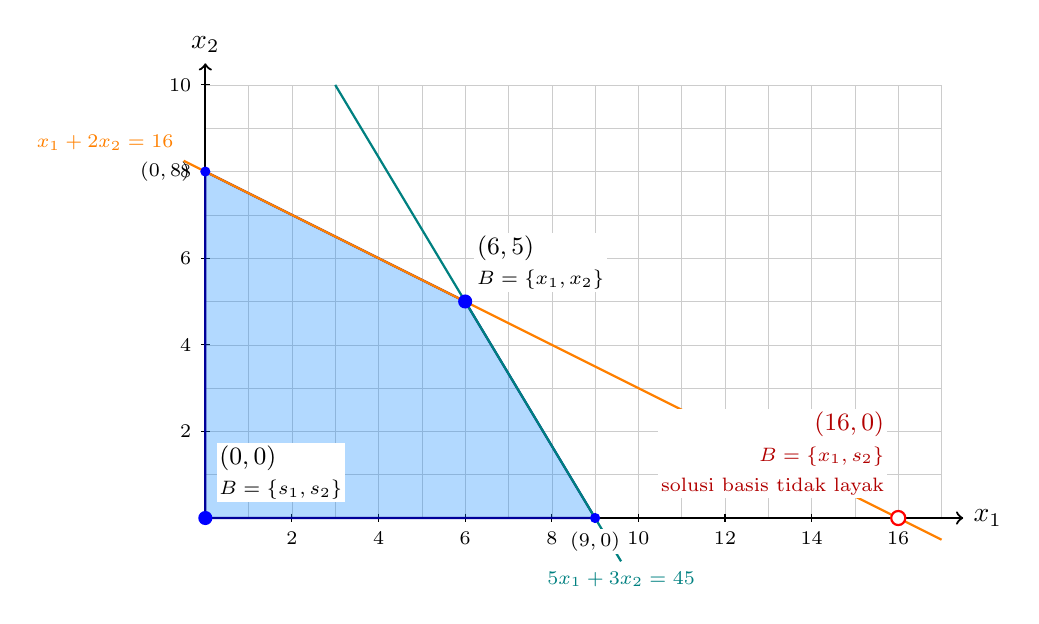
\begin{tikzpicture}[scale=0.55]
    % Grid and axes
    \draw[gray!40, very thin, step=1] (0,0) grid (17,10);
    \draw[->, thick] (0,0) -- (17.5,0) node[right] {$x_1$};
    \draw[->, thick] (0,0) -- (0,10.5) node[above] {$x_2$};
    \foreach \x in {2,4,...,16} \draw (\x,0.1) -- (\x,-0.1) node[below] {\scriptsize \x};
    \foreach \y in {2,4,...,10} \draw (0.1,\y) -- (-0.1,\y) node[left] {\scriptsize \y};

    % Feasible region
    \fill[blue!50!cyan, opacity=0.3] (0,0) -- (9,0) -- (6,5) -- (0,8) -- cycle;
    \draw[blue!60!black, thick] (0,0) -- (9,0) -- (6,5) -- (0,8) -- cycle;

    % Constraint boundaries
    \draw[orange, thick] (-0.5,8.25) node[above left] {\scriptsize $x_1+2x_2=16$} -- (17,-0.5);
    \draw[teal, thick] (3,10) -- (9.6,-1) node[below] {\scriptsize $5x_1+3x_2=45$};

    % Remaining vertices of the region
    \node[fill=blue,circle,inner sep=1.3pt] at (9,0) {};
    \node[anchor=north, fill=white, inner sep=1pt] at (9,-0.25)
        {\scriptsize $(9,0)$};
    \node[fill=blue,circle,inner sep=1.3pt,label={left:\scriptsize $(0,8)$}] at (0,8) {};

    % Basic solutions from the three bases
    \node[fill=blue,circle,inner sep=1.8pt] at (6,5) {};
    \node[anchor=south west, align=left, fill=white, inner sep=1pt]
        at (6.2,5.2) {\small $(6,5)$\\[-1pt]\scriptsize $B=\{x_1,x_2\}$};
    \node[fill=blue,circle,inner sep=1.8pt] at (0,0) {};
    \node[anchor=south west, align=left, fill=white, inner sep=1pt]
        at (0.25,0.35) {\small $(0,0)$\\[-1pt]\scriptsize $B=\{s_1,s_2\}$};
    \node[draw=red,thick,circle,fill=white,inner sep=1.8pt] at (16,0) {};
    \node[anchor=south east, align=right, fill=white, inner sep=1pt,
          text=red!70!black] at (15.75,0.45)
        {\small $(16,0)$\\[-1pt]\scriptsize $B=\{x_1,s_2\}$\\[-1pt]
         \scriptsize solusi basis tidak layak};
\end{tikzpicture}
\end{center}
\caption{Ketiga basis dalam subbagian ini dilihat secara geometris.  Setiap basis menetapkan variabel nonbasis sama dengan nol, sehingga solusi basis terletak pada perpotongan dua batas kendala.  Basis $\{x_1,x_2\}$ dan $\{s_1,s_2\}$ memberikan solusi basis \emph{layak} di titik sudut $(6,5)$ dan $(0,0)$ (titik penuh).  Basis $\{x_1,s_2\}$ memberikan solusi basis $(16,0)$ (titik kosong), yaitu perpotongan sumbu $x_1$ ($x_2=0$) dengan batas $x_1+2x_2=16$ ($s_1=0$); titik ini melanggar $5x_1+3x_2\le 45$, sehingga merupakan solusi basis yang tidak layak dan terletak di luar daerah tersebut.}
\label{fig:matrix-bases-geometry}
\end{figure}

\section{Syarat Optimalitas}
\label{sec:optimality-conditions}
\begin{outcome}
\begin{itemize}
\item Mendefinisikan biaya tereduksi pada suatu solusi basis layak
\item Menetapkan syarat optimalitas melalui biaya tereduksi
\end{itemize}
\end{outcome}
Fungsi objektif program linear diberikan oleh:
    \[
    z = \c^\top \x.
    \]
    Dengan menyubstitusikan variabel yang telah dipartisi, yaitu \( \x_B \) dan \( \x_N \),
    \[
    z =\c_B^\top \x_B +\c_N^\top \x_N.
    \]
    Dengan menyatakan \( \x_B \) dalam \( \x_N \) menggunakan solusi basis \( \x_B = A_B^{-1}\b- A_B^{-1} A_N \x_N \), kita menuliskan ulang fungsi objektif sebagai:
    \begin{equation}
    z =\c_B^\top (A_B^{-1}\b- A_B^{-1} A_N \x_N) +\c_N^\top \x_N.
    \end{equation}
    Dengan menguraikan dan mengelompokkan kembali suku-sukunya:
    \begin{equation}
    z =\c_B^\top A_B^{-1}\b+  (\c_N^\top -\c_B^\top A_B^{-1} A_N )\x_N.
    \end{equation}
    \begin{definition}{Biaya Tereduksi}{}
    Suku \(\c_N^\top -\c_B^\top A_B^{-1} A_N \) merepresentasikan \emph{biaya tereduksi}.  
    
    Ini merupakan objektif yang dituliskan ulang dari sudut pandang suatu solusi basis layak. Secara khusus, komponen-komponen tersebut adalah koefisien variabel nonbasis.
\end{definition}
    

Sistem dituliskan ulang dalam bentuk kamus pada basis $B$ sebagaimana dalam definisi berikut.

\begin{definition}{Kamus Simpleks Terevisi pada Basis $B$}{}
\emph{Kamus simpleks terevisi} pada suatu basis $B$ adalah 
\begin{equation}
\label{eq:dictionary-general}
\begin{aligned}
\max \quad & \mathbf{c}_B^\top A_B^{-1}\mathbf{b} + (\mathbf{c}_N^\top -  \mathbf{c}_B^\top A_B^{-1}A_N)\mathbf{x}_N\\
\st \quad & 
 \mathbf{x}_B 
\;=\;
A_B^{-1}\,\mathbf{b}
\;-\;
A_B^{-1} \,A_N\,\mathbf{x}_N.\\
& \mathbf{x} \geq 0
\end{aligned}
\end{equation}
\end{definition}

Berikut adalah sebuah contoh: program linear yang sama mula-mula ditulis pada basis slack, kemudian pada basis $\{x, y\}$.

\[
\begin{aligned}
\max\quad & 2x + y \\
\st\quad & s_1 = 23 - 3x - y,\\ 
& s_2 = 45 - 5x - 3y,\\ 
& x, y, s_1, s_2 \ge 0.
\end{aligned}
\]

\[
\begin{aligned}
\max\quad & 17 - 0.25s_1 - 0.25s_2 \\
\st\quad & x = 6 - 0.75s_1 + 0.25s_2,\\ 
& y = 5 + 1.25s_1 - 0.75s_2,\\ 
& x, y, s_1, s_2 \ge 0.
\end{aligned}
\]

\begin{theorem}{Syarat Optimalitas dalam Metode Simpleks}{}

    Diberikan suatu program linear dalam bentuk standar:
    \[
    \max \; \c^\top \x \quad \st \quad A \x = b, \quad \x \geq 0,
    \]
    misalkan \(B\) adalah basis yang bersesuaian dengan solusi basis layak \( \x_B = A_B^{-1}\b\), dengan variabel nonbasis \( \x_N = 0 \).

    Jika semua biaya tereduksi memenuhi:
    \[
   \c_N^\top -\c_B^\top A_B^{-1} A_N \leq 0,
    \]
    maka solusi basis layak saat ini bersifat optimal.
\end{theorem}
\begin{proof}
Misalkan $\bar \x = (\bar \x_B, \bar \x_N) = (A_B^{-1}\b, \0)$.

    Jika semua biaya tereduksi bernilai nonpositif, yaitu,
    \[
   \c_N^\top -\c_B^\top A_B^{-1} A_N \leq 0,
    \]
    maka untuk setiap pilihan layak \( \x_N \geq 0 \), 
    kita memperoleh
    \begin{align}
    \c^\top \x &= \c_B^\top A_B^{-1}\b+  (\c_N^\top -\c_B^\top A_B^{-1} A_N )\x_N\\
    &= \c^\top \bar \x +  (\c_N^\top -\c_B^\top A_B^{-1} A_N )\x_N\\
    & \leq \c^\top \bar \x,
    \end{align}
    dengan baris terakhir berlaku karena $(\c_N^\top -\c_B^\top A_B^{-1} A_N ) \leq 0$ dan $\x_N \geq 0$.
    
    Dengan demikian, $\bar \x$ merupakan solusi optimal!
\end{proof}

\label{par:matrix-sign-conventions}%
Catatan tentang konvensi tanda.  Ketiga pembahasan metode simpleks dalam buku ini menyatakan uji optimalitas yang sama dengan tiga cara.  Dalam bentuk kamus pada Bab~\ref{ch:simplex-dictionary}, kita memperbaiki solusi dengan menaikkan variabel nonbasis yang berkoefisien \emph{positif} pada baris objektif, lalu berhenti ketika tidak ada lagi koefisien demikian.  Teorema di atas menyatakan hal yang sama dalam bahasa matriks: koefisien tersebut adalah biaya tereduksi $\c_N^\top -\c_B^\top A_B^{-1} A_N$, dan solusi bersifat optimal ketika semuanya $\leq 0$.  Dalam bentuk tableau pada Bab~\ref{ch:simplex-tableau}, objektif disimpan sebagai persamaan $z - \c^\top\x = 0$, yang membalik tanda koefisien tersebut; karena itu, dalam bentuk ini kita mencari entri baris $z$ yang \emph{negatif} dan berhenti ketika setiap entri bernilai nonnegatif.  Ketiganya merupakan uji yang sama.

\begin{example}{Memverifikasi Optimalitas Menggunakan Biaya Tereduksi}{}

Kita ingin memverifikasi apakah solusi basis layak \( (6,5) \) dan \( (0,8) \) optimal untuk program linear berikut:

\[
\begin{aligned}
    \max \quad & 2 x_1 + 5 x_2 \\
    \st \quad 
    & x_1 + 2x_2 + s_1 = 16, \\
    & 5x_1 + 3x_2 + s_2 = 45, \\
    & x_1, x_2, s_1, s_2 \geq 0.
\end{aligned}
\]
\end{example}

\begin{solution} \textbf{Memeriksa Optimalitas \( (6,5) \)}

\begin{steppanel}{algslate}\cstep{1}{Identifikasi Basis}
Pada titik $(x,y) = (6,5)$, kita melihat bahwa $(s_1, s_2) = 0$.  Dengan demikian, kita dapat memilih 
 \(B= \{x_1, x_2\} \) dan $N = \{s_1, s_2\}$, sehingga:
\[
A_B =
\begin{bmatrix}
    1 & 2 \\
    5 & 3
\end{bmatrix}, \quad
\c_B^\top =
\begin{bmatrix}
    2 & 5
\end{bmatrix}.
\]

Variabel nonbasisnya adalah \( s_1, s_2 \), sehingga:
\[
A_N =
\begin{bmatrix}
    1 & 0 \\
    0 & 1
\end{bmatrix}, \quad
\c_N^\top =
\begin{bmatrix}
    0 & 0
\end{bmatrix}.
\]

\end{steppanel}
\begin{steppanel}{algslate}\cstep{2}{Hitung \( A_B^{-1} \)}
\[
A_B^{-1} =
\frac{1}{(1)(3) - (2)(5)}
\begin{bmatrix}
    3 & -2 \\
    -5 & 1
\end{bmatrix}
=
\begin{bmatrix}
    -3/7 & 2/7 \\
    5/7 & -1/7
\end{bmatrix}.
\]

Dengan demikian, sistem dapat ditulis sebagai 
$$
\x_B = A_B^{-1} \b - A_B^{-1}A_N \x_N,
$$
yaitu
\begin{equation}
\begin{bmatrix} x_1 \\ x_2\end{bmatrix} = \begin{bmatrix} 6 \\ 5\end{bmatrix} - \begin{bmatrix}
    -3/7 & 2/7 \\
    5/7 & -1/7
\end{bmatrix} \begin{bmatrix} s_1 \\ s_2 \end{bmatrix},
\end{equation}
atau secara ekuivalen
\begin{equation}
\begin{bmatrix} x_1 \\ x_2\end{bmatrix} = \begin{bmatrix} 6 \\ 5\end{bmatrix} - s_1 \begin{bmatrix}
    -3/7  \\
    5/7 
\end{bmatrix} - s_2 \begin{bmatrix}
     2/7 \\
    -1/7
\end{bmatrix} 
\end{equation}

\end{steppanel}
\begin{steppanel}{algslate}\cstep{3}{Hitung Biaya Tereduksi}
\[
A_B^{-1} A_N =
\begin{bmatrix}
    -3/7 & 2/7 \\
    5/7 & -1/7
\end{bmatrix}.
\]

\[
\c_N^\top -\c_B^\top A_B^{-1} A_N =
\begin{bmatrix}
    0 & 0
\end{bmatrix}
-
\begin{bmatrix}
    2 & 5
\end{bmatrix}
\begin{bmatrix}
    -3/7 & 2/7 \\
    5/7 & -1/7
\end{bmatrix}.
\]

Dengan menghitung:
\[
\begin{bmatrix}
    0 & 0
\end{bmatrix}
-
\begin{bmatrix}
    (2)(-\tfrac37) + (5)(\tfrac57) & (2)(\tfrac27) + (5)(-\tfrac17)
\end{bmatrix}
=
\begin{bmatrix}
    0 & 0
\end{bmatrix}
-
\begin{bmatrix}
    \tfrac{19}{7} & -\tfrac17
\end{bmatrix}
=
\begin{bmatrix}
    -\tfrac{19}{7} & \tfrac17
\end{bmatrix}.
\]

Biaya tereduksi untuk $s_2$ bernilai positif ($\tfrac17 > 0$), sehingga \( (6,5) \) \emph{tidak} optimal: menaikkan $s_2$ memperbaiki nilai objektif.
\end{steppanel}

\textbf{Memverifikasi Optimalitas \( (0,8) \)}

\begin{steppanel}{algslate}\cstep{1}{Identifikasi Basis}

Pada titik $(x_1, x_2) = (0,8)$, kita memperoleh $s_1 = 16 - 2(8) = 0$ dan $s_2 = 45 - 3(8) = 21$, sehingga variabel basisnya adalah $x_2$ dan $s_2$.  Kita memilih \(B= \{x_2, s_2\} \), sehingga:
\[
A_B =
\begin{bmatrix}
    2 & 0 \\
    3 & 1
\end{bmatrix}, \quad
\c_B^\top =
\begin{bmatrix}
    5 & 0
\end{bmatrix}.
\]

Variabel nonbasisnya adalah \( x_1, s_1 \), sehingga:
\[
A_N =
\begin{bmatrix}
    1 & 1 \\
    5 & 0
\end{bmatrix}, \quad
\c_N^\top =
\begin{bmatrix}
    2 & 0
\end{bmatrix}.
\]

\end{steppanel}
\begin{steppanel}{algslate}\cstep{2}{Hitung \( A_B^{-1} \)}
\[
A_B^{-1} =
\frac{1}{(2)(1) - (0)(3)}
\begin{bmatrix}
    1 & 0 \\
    -3 & 2
\end{bmatrix}
=
\begin{bmatrix}
    \tfrac12 & 0 \\
    -\tfrac32 & 1
\end{bmatrix}.
\]
Sebagai pemeriksaan, $A_B^{-1}\b = \left(\tfrac{16}{2},\, -\tfrac{3}{2}(16) + 45\right) = (8, 21)$, yang sesuai dengan $(x_2, s_2) = (8, 21) \geq 0$: suatu solusi basis layak.

\end{steppanel}
\begin{steppanel}{algslate}\cstep{3}{Hitung Biaya Tereduksi}
\[
A_B^{-1} A_N =
\begin{bmatrix}
    \tfrac12 & 0 \\
    -\tfrac32 & 1
\end{bmatrix}
\begin{bmatrix}
    1 & 1 \\
    5 & 0
\end{bmatrix}
=
\begin{bmatrix}
    \tfrac12 & \tfrac12 \\
    \tfrac72 & -\tfrac32
\end{bmatrix}.
\]

\[
\c_N^\top -\c_B^\top A_B^{-1} A_N =
\begin{bmatrix}
    2 & 0
\end{bmatrix}
-
\begin{bmatrix}
    5 & 0
\end{bmatrix}
\begin{bmatrix}
    \tfrac12 & \tfrac12 \\
    \tfrac72 & -\tfrac32
\end{bmatrix}
=
\begin{bmatrix}
    2 & 0
\end{bmatrix}
-
\begin{bmatrix}
    \tfrac52 & \tfrac52
\end{bmatrix}
=
\begin{bmatrix}
    -\tfrac12 & -\tfrac52
\end{bmatrix}.
\]
\end{steppanel}
Karena kedua biaya tereduksi bernilai negatif, hal ini menegaskan bahwa $(0,8)$ merupakan solusi optimal.

\textbf{Kesimpulan}
\begin{itemize}
\item \( (6,5) \) \emph{tidak optimal} karena memiliki biaya tereduksi yang positif.
\item \( (0,8) \) \emph{optimal} karena semua biaya tereduksinya bernilai nonpositif.
\end{itemize}
\end{solution}

Perhitungan biaya tereduksi yang baru saja kita lakukan merupakan versi aljabar dari gambaran yang layak ditinjau kembali: setiap titik sudut daerah layak memiliki kamusnya sendiri, dan tanda biaya tereduksi menunjukkan apakah terdapat titik tetangga yang lebih baik.  Lihat Gambar~\ref{fig:bfs-perspectives} dalam Bagian~\ref{sec:pivoting} untuk sudut pandang dari satu titik sudut ke titik sudut lainnya tersebut.

\begin{resource}
\begin{itemize}
\item \href{https://www.desmos.com/calculator/j1li4l7lcv}{Desmos: Plot interaktif} suatu PL dari berbagai sudut pandang BFS (\href{https://open-optimization.github.io/open-optimization-or-book/interactive-figures/lp-graphical-method.html}{plot interaktif cadangan}).
\end{itemize}
\end{resource}

\section{Latihan}

\exgroup{Pemanasan}

\begin{ex}{Matriks basis dan solusi basis}{}
\label{ex:matrix-basis-warmup}
\stars{1} Tinjau sistem dari Contoh 1,
\[
\begin{aligned}
    x_1 + 2x_2 + x_3 &= 4, \\
    3x_1 + x_2 + 2x_3 &= 5,
\end{aligned}
\]
dan gunakan basis \( B = \{x_2, x_3\} \).
\begin{enumerate}
    \item Tuliskan matriks basis \( A_B \) dan hitung \( A_B^{-1} \).
    \item Hitung solusi basis \( \x_B = A_B^{-1}\b \) dengan \( x_1 = 0 \).
    \item Apakah solusi basis ini merupakan solusi basis layak?
\end{enumerate}
\exrefs{\S\ref{sec:solutions-axb}, Contoh 1}
\end{ex}

\begin{ex}{Solusi basis yang tidak layak}{}
\label{ex:matrix-infeasible-basis}
\stars{1} Untuk sistem yang sama seperti pada Latihan~\ref{ex:matrix-basis-warmup}, gunakan basis \( B = \{x_1, x_3\} \).  Hitung \( A_B \), \( A_B^{-1} \), dan solusi basisnya, lalu jelaskan mengapa basis ini memberikan solusi basis yang \emph{tidak} layak.
\exrefs{\S\ref{sec:solutions-axb}, Contoh 1}
\end{ex}

\begin{ex}{Basis keempat untuk contoh tiga basis}{}
\label{ex:matrix-fourth-basis}
\stars{1} Dalam Bagian~\ref{sec:three-bases}, kita telah mengevaluasi basis \( \{x_1, x_2\} \), \( \{x_1, s_2\} \), dan \( \{s_1, s_2\} \) dari sistem
\[
\begin{bmatrix}
    1 & 2 & 1 & 0 \\
    5 & 3 & 0 & 1
\end{bmatrix}
\begin{bmatrix}
    x_1 \\ x_2 \\ s_1 \\ s_2
\end{bmatrix}
=
\begin{bmatrix}
    16 \\ 45
\end{bmatrix}.
\]
Sekarang evaluasi basis \( B = \{x_2, s_2\} \): hitung \( A_B \), \( A_B^{-1} \), dan solusi basisnya, lalu tentukan apakah solusi tersebut layak.  Basis ini bersesuaian dengan titik \( (x_1, x_2) \) yang mana?
\exrefs{\S\ref{sec:three-bases}}
\end{ex}

\exgroup{Soal inti}

\begin{ex}{Biaya tereduksi pada dua basis}{}
\label{ex:matrix-reduced-costs}
\stars{2} Tinjau program linear toko roti dari Bagian~\ref{sec:bakery-problem} dalam bentuk standar,
\[
A =
\begin{bmatrix}
1 & 1 & 1 & 0 & 0 \\
2 & 1 & 0 & 1 & 0 \\
1 & 2 & 0 & 0 & 1
\end{bmatrix},
\quad
\b = \begin{bmatrix} 9 \\ 16 \\ 14 \end{bmatrix},
\quad
\c^\top = \begin{bmatrix} 2 & 3 & 0 & 0 & 0 \end{bmatrix},
\]
dengan urutan variabel \( (x, y, s_1, s_2, s_3) \).  Untuk masing-masing basis
\[
B_1 = \{y, s_1, s_2\}
\qquad \text{dan} \qquad
B_2 = \{x, y, s_2\},
\]
hitung \( A_B^{-1} \), solusi basis \( \x_B = A_B^{-1}\b \), nilai objektif \( \c_B^\top A_B^{-1} \b \), dan biaya tereduksi \( \c_N^\top - \c_B^\top A_B^{-1} A_N \).  Gunakan syarat optimalitas untuk menentukan apakah masing-masing basis optimal.
\exrefs{\S\ref{sec:optimality-conditions}, \S\ref{sec:bakery-problem}}
\end{ex}

\begin{ex}{Basis mana yang layak?}{}
\label{ex:matrix-feasible-bases}
\stars{2} Untuk sistem \( 2 \times 4 \)
\[
\begin{bmatrix}
    1 & 2 & 1 & 0 \\
    5 & 3 & 0 & 1
\end{bmatrix}
\begin{bmatrix}
    x_1 \\ x_2 \\ s_1 \\ s_2
\end{bmatrix}
=
\begin{bmatrix}
    16 \\ 45
\end{bmatrix},
\qquad x_1, x_2, s_1, s_2 \geq 0,
\]
terdapat \( \binom{4}{2} = 6 \) cara untuk memilih dua kolom.
\begin{enumerate}
    \item Verifikasi bahwa setiap pasangan dari keenam pasangan kolom saling bebas linear, sehingga setiap pilihan merupakan basis.
    \item Untuk setiap basis, hitung solusi basis dan klasifikasikan sebagai layak atau tidak layak.
    \item Berikan contoh matriks \( 2 \times 4 \) yang memiliki pasangan kolom yang \emph{tidak} membentuk basis.
\end{enumerate}
\exrefs{\S\ref{sec:three-bases}, Gambar~\ref{fig:matrix-bases-geometry}}
\end{ex}

\begin{ex}{Membangun kembali kamus dari rumus}{}
\label{ex:matrix-dictionary-formula}
\stars{2} Bagian~\ref{sec:optimality-conditions} menampilkan program linear
\[
\begin{aligned}
\max\quad & 2x + y \\
\st\quad & 3x + y + s_1 = 23,\\
& 5x + 3y + s_2 = 45,\\
& x, y, s_1, s_2 \ge 0,
\end{aligned}
\]
beserta kamusnya pada basis \( B = \{x, y\} \).  Dengan menggunakan rumus kamus simpleks terevisi~\eqref{eq:dictionary-general}, hitung \( A_B^{-1} \), \( A_B^{-1}\b \), \( A_B^{-1}A_N \), dan biaya tereduksi, lalu pastikan bahwa rumus tersebut menghasilkan kembali kamus yang ditampilkan
\[
\begin{aligned}
\max\quad & 17 - 0.25s_1 - 0.25s_2 \\
\st\quad & x = 6 - 0.75s_1 + 0.25s_2,\\
& y = 5 + 1.25s_1 - 0.75s_2.
\end{aligned}
\]
\exrefs{\S\ref{sec:optimality-conditions}}
\end{ex}

\exgroup{Konsep dan keterkaitan}

\begin{ex}{Biaya tereduksi variabel basis}{}
\label{ex:matrix-basic-reduced-zero}
\stars{2} Vektor biaya tereduksi variabel nonbasis adalah \( \c_N^\top - \c_B^\top A_B^{-1} A_N \).  Terapkan rumus yang sama pada kolom \emph{basis}: tunjukkan bahwa
\[
\c_B^\top - \c_B^\top A_B^{-1} A_B = \0^\top,
\]
sehingga setiap variabel basis memiliki biaya tereduksi tepat nol.  Jelaskan implikasinya terhadap kamus pada basis \( B \): mengapa variabel basis tidak pernah dapat muncul pada baris objektif?
\exrefs{\S\ref{sec:optimality-conditions}}
\end{ex}

\begin{ex}{Tanda biaya tereduksi dan aturan variabel masuk}{}
\label{ex:matrix-sign-conventions}
\stars{2} Dalam bentuk kamus pada Bab~\ref{ch:simplex-dictionary}, variabel masuk adalah variabel nonbasis yang memiliki koefisien \emph{positif} pada baris objektif, sedangkan teorema optimalitas dalam bab ini berhenti ketika semua biaya tereduksi bernilai \( \leq 0 \).
\begin{enumerate}
    \item Jelaskan mengapa keduanya merupakan aturan yang sama: tunjukkan bahwa koefisien variabel nonbasis pada baris objektif suatu kamus \emph{adalah} biaya tereduksinya \( c_j - \c_B^\top A_B^{-1} A_{\{j\}} \).
    \item Biaya tereduksi yang positif menandakan arah perbaikan.  Jelaskan secara geometris apa yang terjadi pada solusi ketika variabel tersebut dinaikkan dari nol.
    \item Sebaliknya, bentuk tableau pada Bab~\ref{ch:simplex-tableau} mencari entri baris \( z \) yang \emph{negatif}.  Dengan menggunakan paragraf konvensi tanda pada \S\ref{par:matrix-sign-conventions}, jelaskan mengapa tidak ada pertentangan.
\end{enumerate}
\exrefs{\S\ref{par:matrix-sign-conventions}, paragraf konvensi tanda; \S\ref{sec:optimality-conditions}}
\end{ex}

\exgroup{Soal tantangan}

\begin{ex}{Biaya tereduksi yang negatif secara ketat menyiratkan optimum unik}{}
\label{ex:matrix-unique-optimum}
\stars{3} Misalkan \( B \) adalah basis suatu PL dalam bentuk standar dengan solusi basis layak \( \bar\x = (A_B^{-1}\b, \0) \), dan andaikan setiap biaya tereduksi bernilai negatif \emph{secara ketat}:
\[
\c_N^\top - \c_B^\top A_B^{-1} A_N < \0^\top \quad \text{(komponen demi komponen)}.
\]
Buktikan bahwa \( \bar\x \) merupakan solusi optimal \emph{unik} dari PL tersebut.  (Ini merupakan suatu argumen, bukan perhitungan.  Rute yang disarankan: ambil sembarang \( \x \neq \bar\x \) yang layak, tulis \( \c^\top \x = \c^\top \bar\x + (\c_N^\top - \c_B^\top A_B^{-1} A_N)\x_N \), lalu tinjau dua kasus \( \x_N = \0 \) dan \( \x_N \neq \0 \).)
\exrefs{\S\ref{sec:optimality-conditions}, teorema Syarat Optimalitas}
\end{ex}

\subsubsection*{Solusi Terpilih}

\begin{solution}(Latihan~\ref{ex:matrix-basis-warmup})
Kolom \( x_2 \) dan \( x_3 \) memberikan
\[
A_B =
\begin{bmatrix}
    2 & 1 \\
    1 & 2
\end{bmatrix},
\qquad
A_B^{-1} = \frac{1}{3}
\begin{bmatrix}
    2 & -1 \\
    -1 & 2
\end{bmatrix}.
\]
Solusi basisnya adalah
\[
\x_B = A_B^{-1}\b = \frac{1}{3}
\begin{bmatrix}
    2 & -1 \\
    -1 & 2
\end{bmatrix}
\begin{bmatrix}
    4 \\ 5
\end{bmatrix}
= \frac{1}{3}
\begin{bmatrix}
    3 \\ 6
\end{bmatrix}
=
\begin{bmatrix}
    1 \\ 2
\end{bmatrix},
\]
sehingga \( (x_1, x_2, x_3) = (0, 1, 2) \).  Kedua variabel basis bernilai nonnegatif, sehingga solusi ini merupakan solusi basis layak.
\end{solution}

\begin{solution}(Latihan~\ref{ex:matrix-reduced-costs})
\textbf{Basis \( B_1 = \{y, s_1, s_2\} \).}  Dengan mengurutkan variabel basis sebagai \( (y, s_1, s_2) \),
\[
A_{B_1} =
\begin{bmatrix}
1 & 1 & 0 \\
1 & 0 & 1 \\
2 & 0 & 0
\end{bmatrix},
\qquad
\x_{B_1} = A_{B_1}^{-1}\b = \begin{bmatrix} 7 \\ 2 \\ 9 \end{bmatrix},
\]
sehingga \( y = 7 \), \( s_1 = 2 \), \( s_2 = 9 \): suatu solusi basis layak dengan nilai objektif \( \c_{B_1}^\top \x_{B_1} = 3 \cdot 7 = 21 \).  Variabel nonbasisnya adalah \( x \) dan \( s_3 \), dan biaya tereduksinya adalah
\[
\c_N^\top - \c_{B_1}^\top A_{B_1}^{-1} A_N = \begin{bmatrix} \tfrac12 & -\tfrac32 \end{bmatrix}.
\]
Biaya tereduksi \( x \) adalah \( \tfrac12 > 0 \), sehingga \( B_1 \) \emph{tidak} optimal; hasil ini sesuai dengan kamus kedua pada Bab~\ref{ch:simplex-dictionary}, \( z = 21 + \tfrac12 x - \tfrac32 s_3 \).

\textbf{Basis \( B_2 = \{x, y, s_2\} \).}  Di sini
\[
A_{B_2} =
\begin{bmatrix}
1 & 1 & 0 \\
2 & 1 & 1 \\
1 & 2 & 0
\end{bmatrix},
\qquad
\x_{B_2} = A_{B_2}^{-1}\b = \begin{bmatrix} 4 \\ 5 \\ 3 \end{bmatrix},
\]
suatu solusi basis layak dengan nilai \( 2 \cdot 4 + 3 \cdot 5 = 23 \).  Variabel nonbasisnya adalah \( s_1 \) dan \( s_3 \), dengan biaya tereduksi
\[
\c_N^\top - \c_{B_2}^\top A_{B_2}^{-1} A_N = \begin{bmatrix} -1 & -1 \end{bmatrix} \leq \0^\top,
\]
sehingga \( B_2 \) optimal, sesuai dengan kamus terakhir \( z = 23 - s_1 - s_3 \).
\end{solution}

\begin{solution}(Latihan~\ref{ex:matrix-unique-optimum})
Tuliskan \( \bar{\c}_N^\top = \c_N^\top - \c_B^\top A_B^{-1} A_N \) dan \( z^* = \c^\top \bar\x = \c_B^\top A_B^{-1} \b \).  Setiap \( \x \) yang layak memenuhi \( A_B \x_B + A_N \x_N = \b \), sehingga \( \x_B = A_B^{-1}\b - A_B^{-1}A_N \x_N \) dan, tepat seperti dalam teorema optimalitas,
\[
\c^\top \x = z^* + \bar{\c}_N^\top \x_N .
\]
Ambil sembarang \( \x \neq \bar\x \) yang layak.

\emph{Kasus 1: \( \x_N \neq \0 \).}  Maka terdapat komponen \( x_j > 0 \) dengan \( j \in N \), dan karena setiap entri \( \bar{\c}_N \) bernilai negatif secara ketat, \( \bar{\c}_N^\top \x_N < 0 \).  Akibatnya, \( \c^\top \x < z^* \), sehingga \( \x \) tidak optimal.

\emph{Kasus 2: \( \x_N = \0 \).}  Maka \( A_B \x_B = \b \), dan karena \( A_B \) dapat diinvers, hal ini memaksa \( \x_B = A_B^{-1}\b \), yaitu \( \x = \bar\x \), yang bertentangan dengan \( \x \neq \bar\x \).

Oleh karena itu, setiap titik layak selain \( \bar\x \) memiliki nilai objektif yang lebih kecil secara ketat daripada \( z^* \): solusi \( \bar\x \) optimal dan tidak ada solusi optimal lain.
\end{solution}
